\chapter{How to Manage Stress and Mental Health?}

This chapter comes from a short School of Hard Knocks entrepreneurship interview curated by LazyingArt LLC. The exchange is practical rather than formal: the interviewer asks how a person in demanding positions manages mental health, stress, and work-life balance, and the answer unfolds as a small operating model for sustained work. We will keep the speaker's order: first the problem, then the principle of having more than one focus, then the morning rhythm, then hobbies, and finally the old image of sharpening the axe.

\section{The Question: Stress Inside Demanding Roles}

The opening question is not about leisure in the abstract. It asks how stress is managed while one is still carrying responsibility. That matters because entrepreneurship often rewards focus, persistence, and intensity, but those same virtues can become brittle if the whole life is reduced to the office.

The question can be written as a very simple tension:
\begin{equation}
\hbox{demanding role}+\hbox{continuous pressure}
\quad \Longrightarrow \quad
\hbox{stress risk}.
\end{equation}
This is not a formal law. It is the situation the answer is trying to resolve. The speaker's resolution begins with a principle: one has to have more than one focus in life.

\section{More Than One Focus}

The first move is to reject a single-focus model of life. In the speaker's answer, balance does not begin as a calendar trick. It begins as a diversification of attention:
\begin{equation}
\mathcal{F}
=
\{\hbox{work},\ \hbox{training},\ \hbox{hobbies}\}.
\end{equation}
The notation is ours, but it captures the spoken structure. Work remains present, but it is not the only domain in which the person exists.

\subsection{Question \& Answer}

\paragraph{Question.}
If the business, the office, or the position matters so much, why deliberately maintain other focuses?

\paragraph{Answer.}
Because a person is not just the hours directly spent producing. The speaker's claim is that other domains give back mental space, distance, and renewal. In entrepreneurial terms, they maintain the operator. A work life organized around only work may look intense in the short run, but it has no explicit mechanism for recovery.

We can express the cautious mechanism this way:
\begin{equation}
O_{\mathrm{sustained}}
\sim
E_{\mathrm{work}}\cdot C_{\mathrm{maintained}},
\end{equation}
where \(O_{\mathrm{sustained}}\) is durable output, \(E_{\mathrm{work}}\) is direct work effort, and \(C_{\mathrm{maintained}}\) is the maintained capacity of the person doing the work. The equation is a bookkeeping device, not a transcript quotation.

\section{The Morning Rhythm}

The answer then turns concrete. The speaker gives a rhythm rather than a slogan: he gets up at 4:30 in the morning and is in the gym by 5. The times are important because they show that the principle is not left floating.

\begin{align}
t_{\mathrm{wake}} &= 4{:}30\ \mathrm{a.m.},\\
t_{\mathrm{gym}} &= 5{:}00\ \mathrm{a.m.}.
\end{align}

The workout frequency is also stated concretely. He generally works out seven days a week; some weeks it is six, and some days include two workouts:
\begin{align}
f_{\mathrm{workout}} &\approx 7\ \hbox{days/week},\\
f_{\mathrm{workout}} &\approx 6\ \hbox{days/week}\quad \hbox{on some weeks},\\
n_{\mathrm{workouts/day}} &= 2\quad \hbox{on some days}.
\end{align}
This should not be turned into a universal command to copy the same schedule. It is evidence of the speaker's personal system: recovery and discipline are scheduled before the office can consume the day.

\section{Mind Space And Self-Directed Goals}

The speaker next explains why the gym matters. It gives him mind space. It is a place where he is working toward goals in a domain outside the office.

This is the important transition. The gym is not merely exercise. In the logic of the answer, it is a separate control loop:
\begin{equation}
\hbox{training}
\quad \Longrightarrow \quad
\hbox{mind space}+\hbox{self-directed goals}.
\end{equation}
That is why the routine belongs in a chapter on entrepreneurial judgment. The point is not that every founder must train seven days a week. The point is that the speaker has built a non-office arena where effort, progress, and attention are still his own.

\begin{figure}
\centering
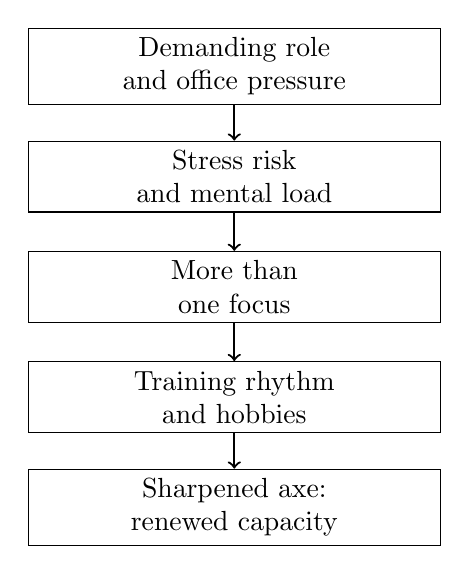
\begin{tikzpicture}[x=1cm,y=1cm]
\node[draw, rectangle, align=center, text width=5.0cm] (role) at (0,0) {Demanding role\\and office pressure};
\node[draw, rectangle, align=center, text width=5.0cm] (risk) at (0,-1.4) {Stress risk\\and mental load};
\node[draw, rectangle, align=center, text width=5.0cm] (focus) at (0,-2.8) {More than\\one focus};
\node[draw, rectangle, align=center, text width=5.0cm] (practice) at (0,-4.2) {Training rhythm\\and hobbies};
\node[draw, rectangle, align=center, text width=5.0cm] (capacity) at (0,-5.6) {Sharpened axe:\\renewed capacity};

\draw[->, thick] (role) -- (risk);
\draw[->, thick] (risk) -- (focus);
\draw[->, thick] (focus) -- (practice);
\draw[->, thick] (practice) -- (capacity);
\end{tikzpicture}
\caption{A transcript-derived reconstruction of the answer's logic: stress is met by maintaining more than one focus, not by pretending the office is the whole life.}
\end{figure}

\section{Hobbies As Distance From The Office}

The next pivot is simple: ``And then I also have hobbies.'' The speaker lists golf, sailing, hiking, and road biking. The list is plain, but its function is precise. These are ways to get away from the office.

\begin{table}
\centering
\begin{tabular}{p{0.32\linewidth} p{0.52\linewidth}}
\hline
Domain & Function in the answer \\
\hline
Gym rhythm & Mind space and a separate goal arena \\
Hobbies & Distance from the office environment \\
Office work & The demanding role that must be sustained \\
\hline
\end{tabular}
\caption{The speaker's examples divide life into distinct domains, each with a different role in maintaining capacity.}
\end{table}

The draft should preserve the humility in the golf example: he says he does not play very well, but he likes to play. That small detail matters. The point is not mastery or status. The point is a living domain outside the office.

\section{Sharpening The Axe}

The closing move is the Abraham Lincoln anecdote: if he had four hours to chop down a tree, he would spend the first three sharpening the axe. The interview uses this as an image of preparation and maintenance.

As a ratio, the anecdote is:
\begin{align}
T_{\mathrm{total}} &= 4\ \hbox{hours},\\
T_{\mathrm{sharpen}} &= 3\ \hbox{hours},\\
T_{\mathrm{chop}} &= 1\ \hbox{hour}.
\end{align}
So the preparation share is:
\begin{equation}
\frac{T_{\mathrm{sharpen}}}{T_{\mathrm{total}}}
=
\frac{3}{4}.
\end{equation}
We should not over-literalize this ratio. The speaker is not proposing that three quarters of every workday be spent away from work. He is giving a compact rule of judgment: the act of maintaining the tool is part of the work.

\subsection{A Bookkeeping Example}

To see the mechanism without pretending it is a scientific measurement, suppose daily capacity is represented by \(C_n\). Stress draws it down, and recovery practices rebuild it:
\begin{equation}
C_{n+1}=C_n-S_n+R_n.
\end{equation}
Here \(S_n\) is the strain from the day, and \(R_n\) is recovery from training, hobbies, and distance from the office.

A week with no recovery has the schematic form:
\begin{equation}
C_7=C_0-\sum_{n=0}^{6}S_n.
\end{equation}
A week with regular recovery has:
\begin{equation}
C_7=C_0-\sum_{n=0}^{6}S_n+\sum_{n=0}^{6}R_n.
\end{equation}
This is the mathematical skeleton of the speaker's practical claim. The gym, golf, sailing, hiking, and road biking are not distractions in this model. They are terms in \(R_n\), the part of the system that keeps the person able to keep working.

\section{Summary}

The answer begins with stress and work-life balance, but it does not end with a vague appeal to relaxation. It gives a sequence: have more than one focus, make the rhythm concrete, protect mind space, maintain hobbies that create distance from the office, and treat those practices as sharpening the axe.

The chapter's durable lesson is that entrepreneurial capacity is maintained, not merely spent. Direct work matters, but the person doing the work is also part of the operating system.